
\section{Big picture}
 
Examining stimulus-response data and extrapolating from that a model
that allows us to predict, given a set of responses, what the stimulus 
likely was.  Still working on this section.........



%---------This should be more general and give a big picture-------------
%----what do you want to accomplish?
%----what is neural activity in general?
%-----why is a low dim model important?
%-----is idea to understand how the brain is working?
%------How is the brain coding information?
%------how can we decode information based on brain activity?
%----what consequences would there be if we found a low dimensional structure?
%----what is the relevance of having a similarity measure?
%-----e.g want to know whether the brain is thinking about similar things 
%----at different brain states/instances
%----why?  --- what does this have to do with the structure of the space



\section{Biological background}
\subsection{Structure of a neuron}
A neuron is a specialized cell in the nervous system that receives, represents, and transmits information through a series of electrical pulses called action potentials or spikes. The neuron is the fundamental unit of brain function and is made of three major parts: the dendrites (which receive information from other neurons), the cell body or soma (which processes information) and the axon (which transmits information to other neurons) (Figure \ref{fig:Neuron}).

\begin{figure}[h]
\centering
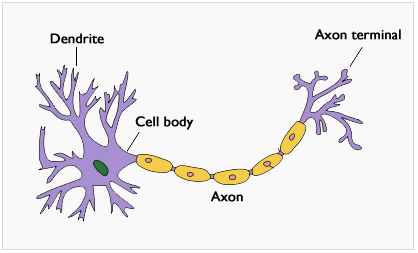
\includegraphics[width=\textwidth]{/home/tesylvia/Oral_Sept_2017/images/Neuron.jpg}
%label the figure so latex can reference it
\caption{Structure of  a neuron, please cite your source......}
      \label{fig:Neuron}
\end{figure}


The cell membrane is made up of phospholipids (fat) and separates the cell interior from the extracellular space. The lipid cell membrane is impermeable
to charged ions but thin enough to allow interaction of separated charged
ions through electrostatic forces. Thus the cell membrane acts as an electrical
capacitor. Embedded in the cell membrane are Na$^{+}$ (sodium) and K$^{+}$ (potassium) ion exchange pumps which pump out three Na$^{+}$ ions for every two K$^{+}$ ions pumped in. As a result, Na$^{+}$ is more concentrated outside the cell than inside it, and the intracellular concentration of K$^{+}$ is substantially higher than that outside the cell. There are gated ion channels
(trans-membrane proteins) embedded in the cell membrane which open or close enabling predominantly K$^{+}$, Na$^{+}$, Ca$^{2+}$ (calcium), and Cl$^{-}$ (chloride) ions to flow into and out of the cell. The ion channels act as conductors.

\subsection{Membrane potential}
A potential is a distribution of charge across the cell membrane.
\textit{Voltage} is a measure of the potential energy generated by separated charges and is measured in millivolts (mV). Ions flow into and out of the cell due to both voltage and concentration gradients. \textit{Current} refers to the flow of charged ions into and out of the cell. A resting neuron contains a greater number of negative charges on the inside than on the outside. 
This difference in separated charges is called the neuron's \textit{membrane potential}. A neuron with a membrane potential of approximately -70mV is called \textit{polarized}. This number is also referred to as the resting membrane potential.  

\subsection{Generation of an action potential}
Dendrites contain chemically-gated ion channels, which open when 
a stimulus affects a sensory receptor, such as neurotransmitters binding to the dendrite receptors. As a result, current flows into the intracellular fluid, causing the membrane potential to be less negative or to be positive (depolarization of the neuron). 
This increase in the membrane potential causes the voltage-gated Na$^{+}$ channels, at the entry point of the axon, to open and thus more Na$^{+}$ flows into the cell down its electrochemical  gradient. When a certain threshold is reached ($\approx$ -55mV), an electrical pulse lasting  a short duration ($\approx$ 1ms),  called an \textit{action potential}, is released and is propagated over long distances along the neuron's axon. When the membrane potential rises, the voltage-gated K$^{+}$ channels open, allowing more K$^{+}$ to flow out of the cell, which causes the membrane potential to fall below the resting potential (hyperpolarization of the neuron). The neuron later returns to its resting potential after a refractory period, during which the likelihood of spiking is greatly reduced. The axon terminal contains voltage-gated Ca$^{2+}$ channels which open causing an influx of Ca$^{2+}$. This leads to the release of 
neurotransmitters (stored in the synaptic vesicles) into the synaptic cleft.
The neurotransmitters then bind to the dendrite receptors of nearby neurons.
A synapse is a specialized structure that facilitates communication between neurons. The neuron that sends off an action potential is called \textit{presynaptic} and the one receiving the chemical message is called a \textit{postsynaptic} neuron. Depending on the chemical properties of the binding neurotransmitters, action potentials fall into two broad categories. Excitatory post synaptic potentials (EPSP) result from excitation of a postsynaptic neuron, while inhibitory post synaptic potentials (IPSP) result from inhibition.

\subsection{Measuring neurons}
The electrical properties of biological cells are measured using electrodes, which allow electrical current to pass through them when they come into contact with electrolytes. Due to the small size of cells, microelectrodes are typically used to measure single unit spiking activity.
A \textit{single unit} refers to a single action potential-generating neuron, whose spikes are clearly isolated by a recording microelectrode \cite{Humphrey1990}.
Neurons are measured using two methods: \textit{intracellular recording}, a process where an electrode is inserted inside the cell body and \textit{extracellular recording} in which an electrode is inserted in the extracellular space near the cell body. (Figure \ref{fig:Electrodes}).
Intracellular electrodes record membrane potential by comparing the potential on the inserted electrode to that of a reference electrode placed in the extracellular fluid surrounding the cell body. Extracellular recordings can be 
processed (via spike sorting algorithms) to obtain spike times.

\begin{figure}[h]
\centering
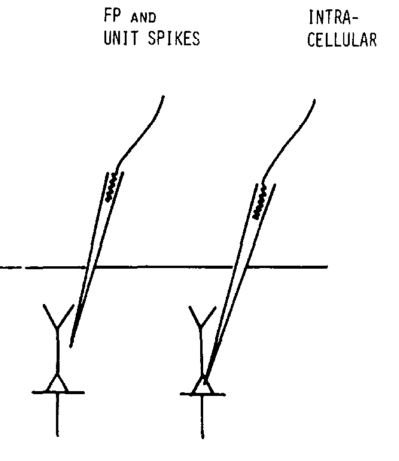
\includegraphics[width=3in]{/home/tesylvia/Oral_Sept_2017/images/MeasuringNeuron.png}
\caption{Intracellular and  extracellular recordings, adapted from figure 2 of \cite{Humphrey1990}.}
%label the figure so latex can reference it
      \label{fig:Electrodes}
\end{figure}

Multi-electrode arrays enable simultaneous single-unit recordings from multiple brain sites. The data set we analyze is based on extracellular multiple single-unit single-trial recordings in which spike times of single units have been isolated using suitable spike sorting algorithms.


\subsection{Place cells and place fields}
Place cells are neurons found in the CA1 and CA3 region of the rat hippocampus,
whose firing rate is strongly modulated by the position of the rat within it's
environment. Hence place cells appear to be encoding location \cite{OKeefe1971, OKeefe1978}. The region where a place cell is highly likely to spike is called a place field.

\subsection{Spike trains} 
Experimentalists obtain information that neurons carry about an organism's
environment by measuring from neurons. Spike trains are considered as the 
main mode of information transmission in the nervous system. 
A spike train is an ordered sequence of recorded times at which a neuron
fires an action potential (spike) \cite{Dayan2001}.


\subsection{Raster plot}
A raster plot is a graphical representation of spike trains. In this graph,
a short vertical line is used to show the time at which a spike occurred
in a recorded voltage trace.
Figure \ref{fig:Raster} shows a raster plot of real-world data
from the CA1 region of the rat hippocampus. The y-axis represents the neuron
label while the x-axis represents spike times.\\
 \begin{figure}[H]
  \centering
    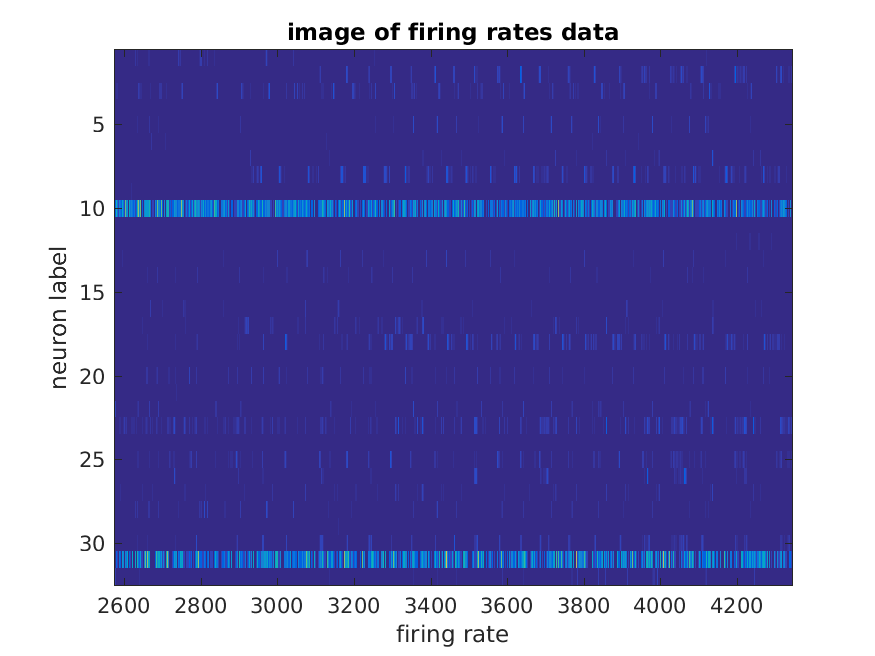
\includegraphics[scale=0.5]{/home/tesylvia/Oral_Sept_2017/images/RasterPlot.png}
     \caption{Raster plot for real-world data from a rat hippocampus provided by the Redish Lab}
     %label the figure so latex can reference it
      \label{fig:Raster}
\end{figure}

The goal of our analysis is to investigate the relationship between
spike trains (neural activity) and other variables such as stimuli and location.
It is known that place cell firing is closely correlated with the animal's location in it's environment \cite{OKeefe1971, OKeefe1978, Burgess1994}.



\subsection{Poisson processes}
We represent a spike train as a sequence of random events, that is, as a point process where the random events correspond to spike times. We focus on the simplest point process: a Poisson process, where the numbers of events in non-overlapping intervals are independent random variables. If the probability per unit time (the instantaneous event rate r) is constant, the Poisson process is 
called a \textit{homogeneous Poisson process}. On the other hand if the instantaneous firing rate varies with time, the Poisson process is called a 
\textit{non-homogeneous Poisson process}.



















































%=========================================================================================


%=======Below was my original objective===================================================
%The objective of this present project is to find a low dimensional model of interactions, among a subtype of neurons called place cells, in the CA1 region of the rat hippocampus, believed to be specified to relay the animal's physical position. The model is extrapolated from application of a non-linear dimensionality tool called diffusion maps, to a designed 
%similarity matrix of activity patterns.\\



%======================Gaussian Processes below for future works==============================
%\newpage
%\section{Linear dimensionality reduction techniques}
%\subsection{Gaussian Process Factor analysis}
%\begin{Def}
%A vector-valued random variable $\vect{X} = \left[x_{1}, \ldots , x_{n} \right]^T$
%has a multivariate Gaussian distribution if it's  probability density function is given by
%   
%\[
%f(\vect{x})  = (2\pi)^{-\frac{n}{2}} \det({\Sigma})^{-\frac{1}{2}} 
%\exp \bigg( -\frac{1}{2}(\vect{x - \mu})^{T}\Sigma^{-1}(\vect{x - \mu}) \bigg)
%\]
%
%with mean vector  $\vect{\mu} \in \mathbb{R}^n$ and covariance matrix $\Sigma$.
%The covariance matrix must be a positive semidefinite (PSD) matrix for such a density to exist.
%We write $X  \sim N(\vect{\mu}, \Sigma).$
%
%\end{Def}
%
%
%\begin{Def} A Gaussian Process (GP) is a Gaussian distribution over functions \\
%$f: \mathbb{R}^n \rightarrow   \mathbb{R}^n$  defined by specifying a mean
%function $m: \mathbb{R}^n \rightarrow \mathbb{R}$  and a kernel
%$K: \mathbb{R}^n  \times \mathbb{R}^n \rightarrow \mathbb{R} $ such that the following
%conditions hold:
%
%\begin{itemize}
%\item each vector valued random variable 
%$f(\vect{t}) = \left[f(t_1), \ldots , f(t_n) \right]^T$ has a multivariate Gaussian distribution for all  
%$\vect{t} = \left[t_1, \ldots, t_n   \right]^T$, that is, 
%$f(\vect{t}) \sim  N(m(\vect{t}), K(\vect{t}, \vect{t})).$
%
%\item $m(\vect{t}) = \E(f(\vect{t}))$
%
%\item $K(\vect{t},\vect{s}) = \E\left[ \big(f(\vect{t}) - m(\vect{t}) \big) \big( (f(\vect{s}) - m(\vect{s}) \big)^T   \right]$  for any $\vect{t}, \vect{s} \in \R^n.$  
%
%\item K satisfies the Mercer theorem.
%
%\end{itemize}
%\end{Def}
%
%\begin{Thm}
%
%Every matrix $ K(\vect{t}, \vect{t}) = \{ K(t_i, t_j) \}_{1 \leq i, j \leq n} = (k_{ij}) $
%is a PSD  for all time $\vect{t}$ if
%\[  \vect{v}^T K \vect{v} = 
%\sum_{i=1}^{n} \sum_{j=1}^{n} k_{ij} v_i v_j =
% \sum_{i=1}^{n} \sum_{j=1}^{n} k(t_i, t_j) v_i v_j \geq 0  
% \quad \text{for all}  \quad \vect{v}  \neq \vect{0}. \] 
%
%\end{Thm}
%
%
%\begin{Ex}
%One of the most commonly used kernels is the squared exponential kernel (SE) given by
%$K(t_{i}, t_{j}) = \sigma_{f}^{2} \exp \{-\frac{1}{2l^2}  (t_i - t_j)^2 \}$
%where $\sigma_{f}^{2}$  is the variance of the kernel and l is the length scale.
%
%\end{Ex}
%



%============================================================================================
%%======How to insert a table in latex===================%

%\begin{table}[H]
%   \centering
%    \begin{tabular}{|c|c|c|c|}\hline
%    $x$ & 0 & 1 & 2\\ \hline
%    $f(x)$ & 3 & 6 & 9\\ \hline
%    \end{tabular}
%     \caption{Caption goes here}
%\end{table}

%%=====end table==================================%
%\begin{figure}[H]
%  \centering
%    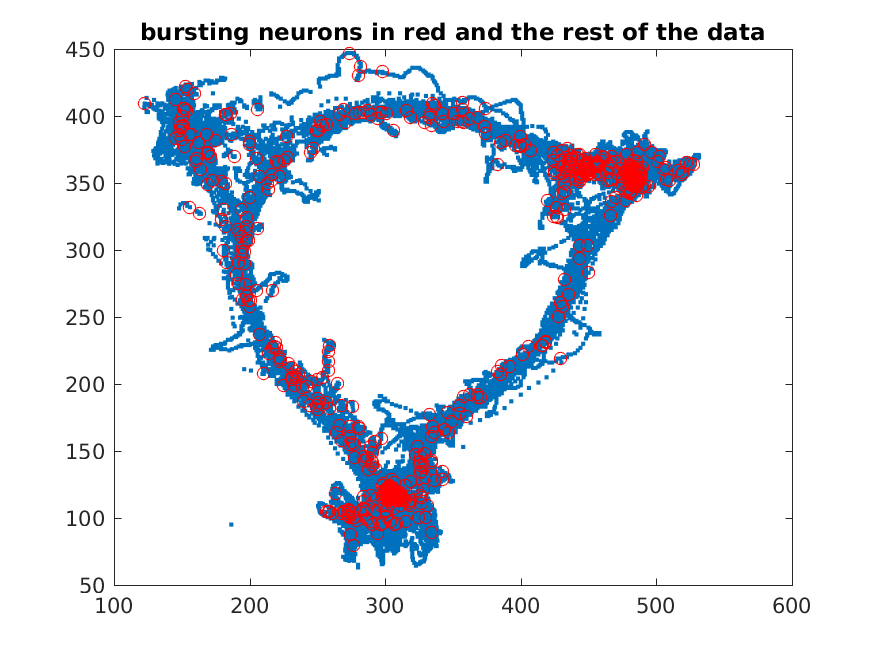
\includegraphics[scale=0.5]{Bursting_neuron.png}
%     \caption{The bursting neuron}
%      \label{tab:data1}
%\end{figure}


%===========Insert a figure in latex=============%






%============end figure===========================%

%\begin{itemize}
%\item What is the nature of the problem you're trying to solve?
%\item Two most well known models that inspired your work
%\item The authors and names of these models
%\item What were they modeling?
%\item Strengths and weaknesses of these models
%\item Overview of our model
%\item What is promising about our model
%\item why are you going to use dimensionality reduction to study the model
%\item why use vector space embeddings instead of the point process framework
%\item Report any results that may be significant and supported by a measure of "goodness"
%\item Mention that this is the first time this type
%of analysis has been applied to the Redish Lab data 
%obtained from the CA1 region of the Hippocampus
%\end{itemize}

